\section{User Study}\label{sec:user-study}
{We next conduct user studies to assess whether and how humans exhibit biases when responding to algorithms. We use the results of these experiments as a proof of concept, shedding light on the existence of misperceptions about algorithm explanations in real-world scenarios, and show that they can be interpreted using our model of feature weight misperceptions. These user studies also help us understand the conditions where our model performs well, as well as settings where our model has shortcomings.}

\subsection{Study Design, Participants, and Setup}\label{sec:study-design}
To understand how human biases affect their responses to algorithms, we conducted a large-scale online survey where participants completed a task with an optimal solution (here, an optimal strategic response to a classifier). We then measured how their answers differed from the optimal solution to assess bias. Similar to previous sections, we focus on how participants perceive the feature weights and how this influences their response to the algorithm. Surveys generally took {5.5} minutes, and participants were paid {\$16 per hour}. The study design was reviewed by our IRB, and the full protocol is included in the supplementary materials. 

\noindent\textbf{Experimental Design.} We used a $2\times2$ between-subjects design, varying the number of features and the feature weights and two contexts. Participants were randomly assigned to a condition and shown a single explanation (shown in Figure~\ref{fig:feature-based-explanations}), with \textit{a}) either two or four features, \textit{b}) either balanced or unbalanced feature weights, and \textit{c}) either familiar or unfamiliar context. 

\noindent\textbf{Procedure.} All participants were shown a truthful and complete explanation from an interpretable ML algorithm. Each participant was asked to complete a task based on the information provided in the explanation. After completing the task, participants were asked questions about their understanding, trust, satisfaction, and performance, common measures in explainability evaluations~\cite{mohseni2021survey}. 

\noindent\textbf{Explanation.} Based on prior work, which has found that feature importance is the most used explanation \cite{systematic2023nauta} and that visualization can help users understand explanations \cite{peeking2018adadi}, we developed an explanation that shows feature weights in a bar graph (Figure~\ref{fig:feature-based-explanations}). The system uses the displayed feature weights as an interpretable ML algorithm. 

\begin{figure*}[ht]
    \centering 
    %KV CHANGED SO ALL IMAGES SAME WIDTH 
    \hspace{.5em}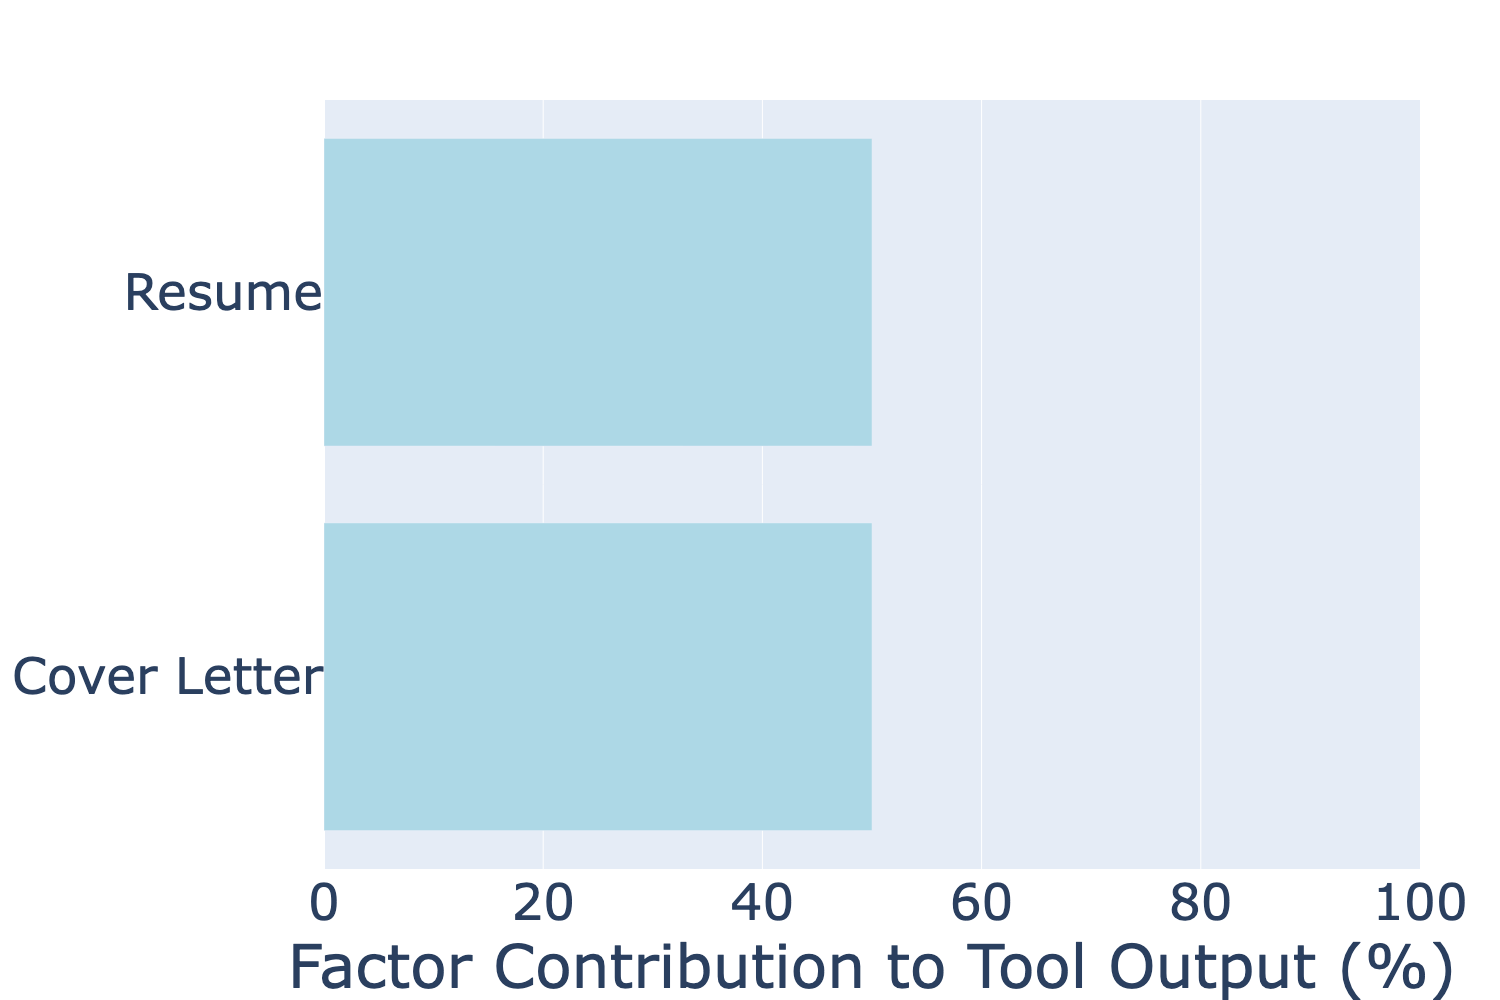
\includegraphics[width=0.245\textwidth]{Figures/2-equal.png}
    \hspace{.5em}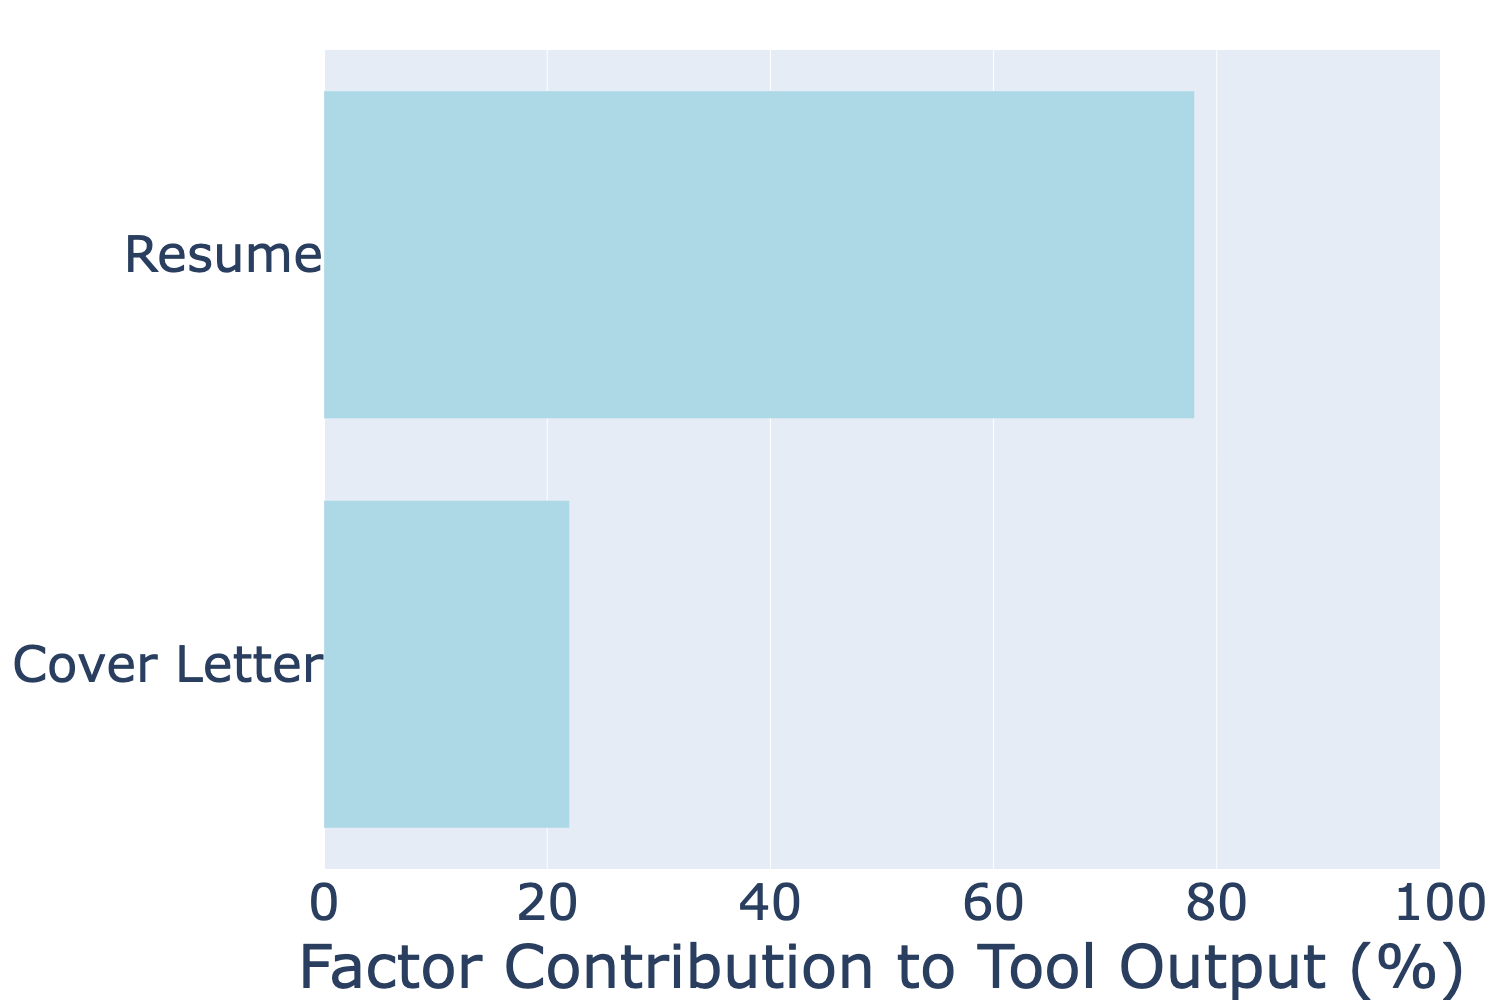
\includegraphics[width=0.24\textwidth]{Figures/2-unequal.png}
    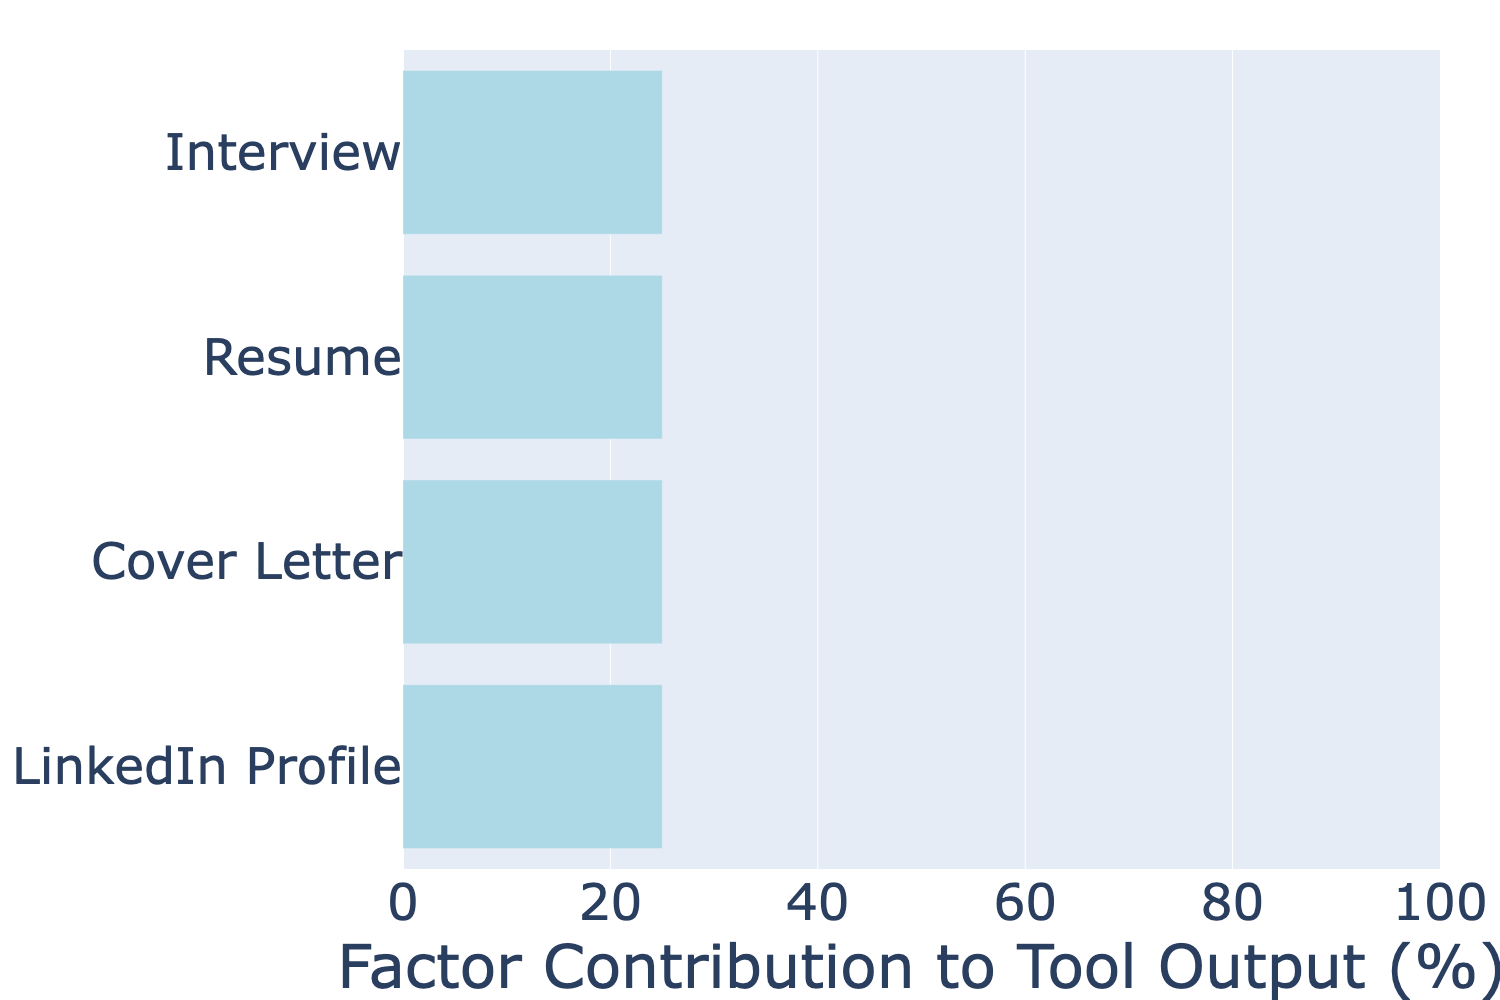
\includegraphics[width=0.24\textwidth]{Figures/4-equal.png}
    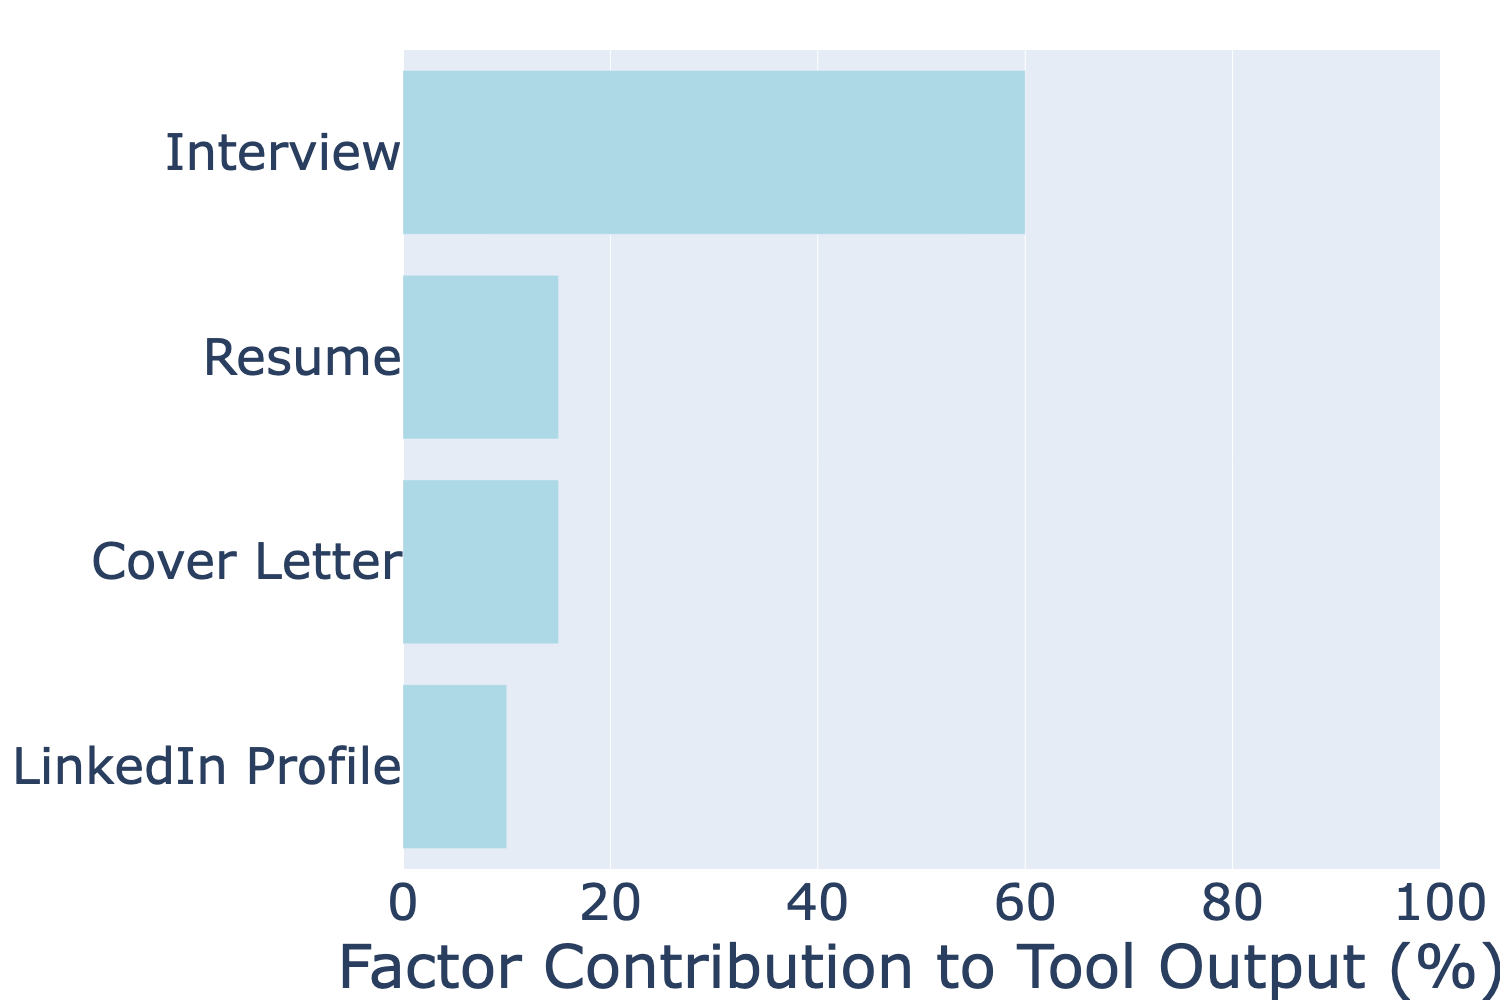
\includegraphics[width=0.24\textwidth]{Figures/4-unequal.png}\\
    \hspace{.5em}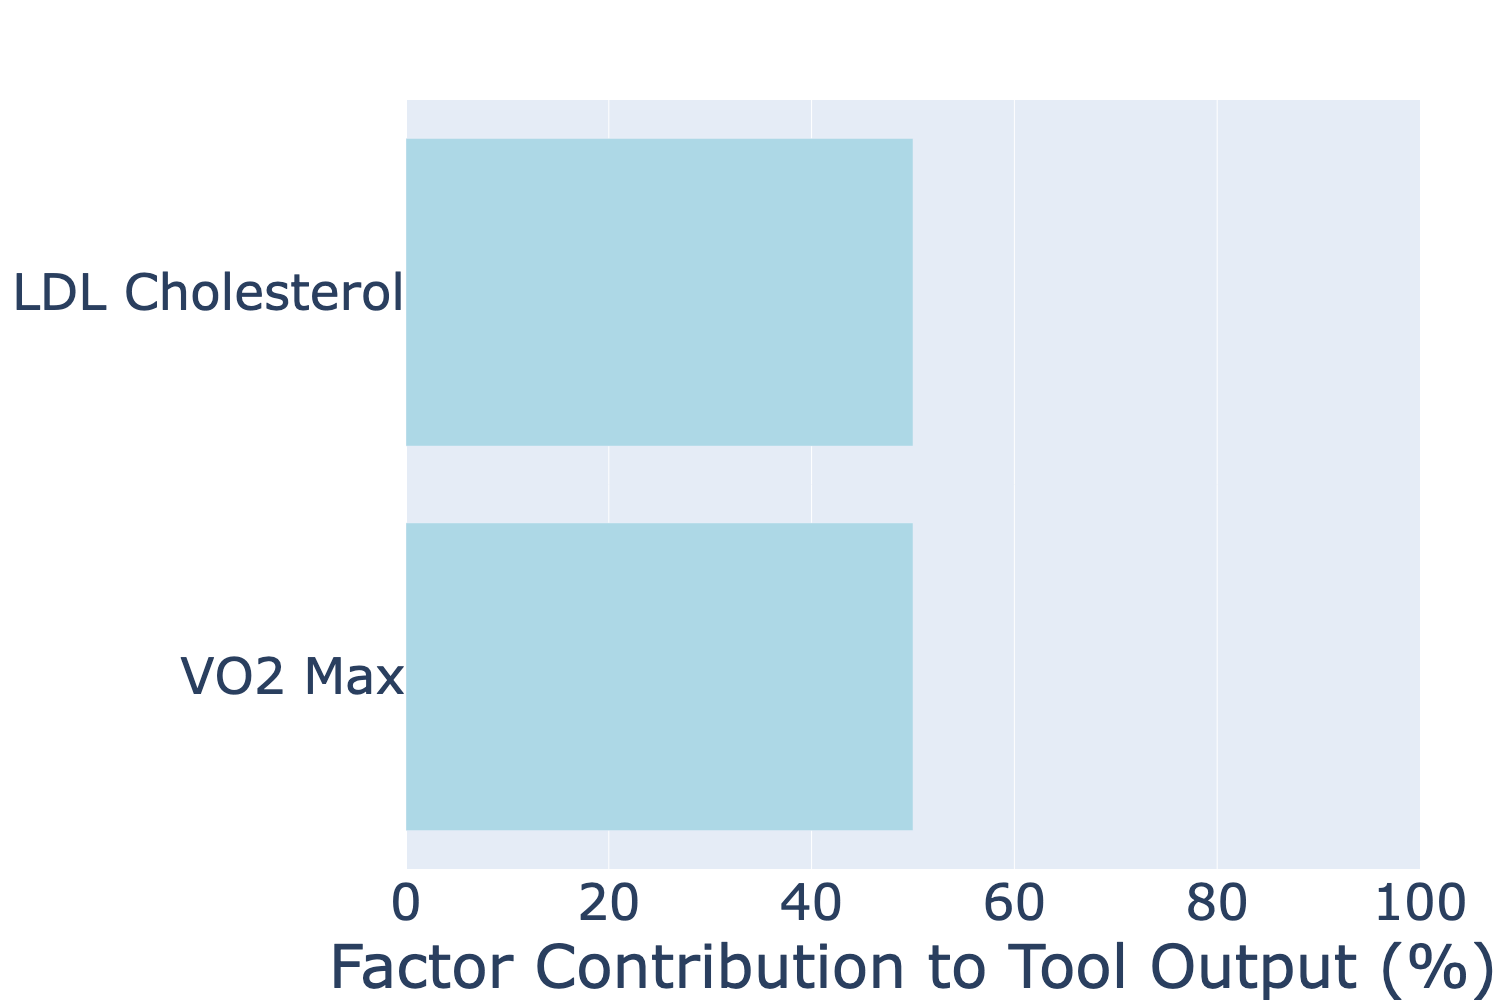
\includegraphics[width=0.245\textwidth]{Figures/2_unf_bal.png}
    \hspace{.5em}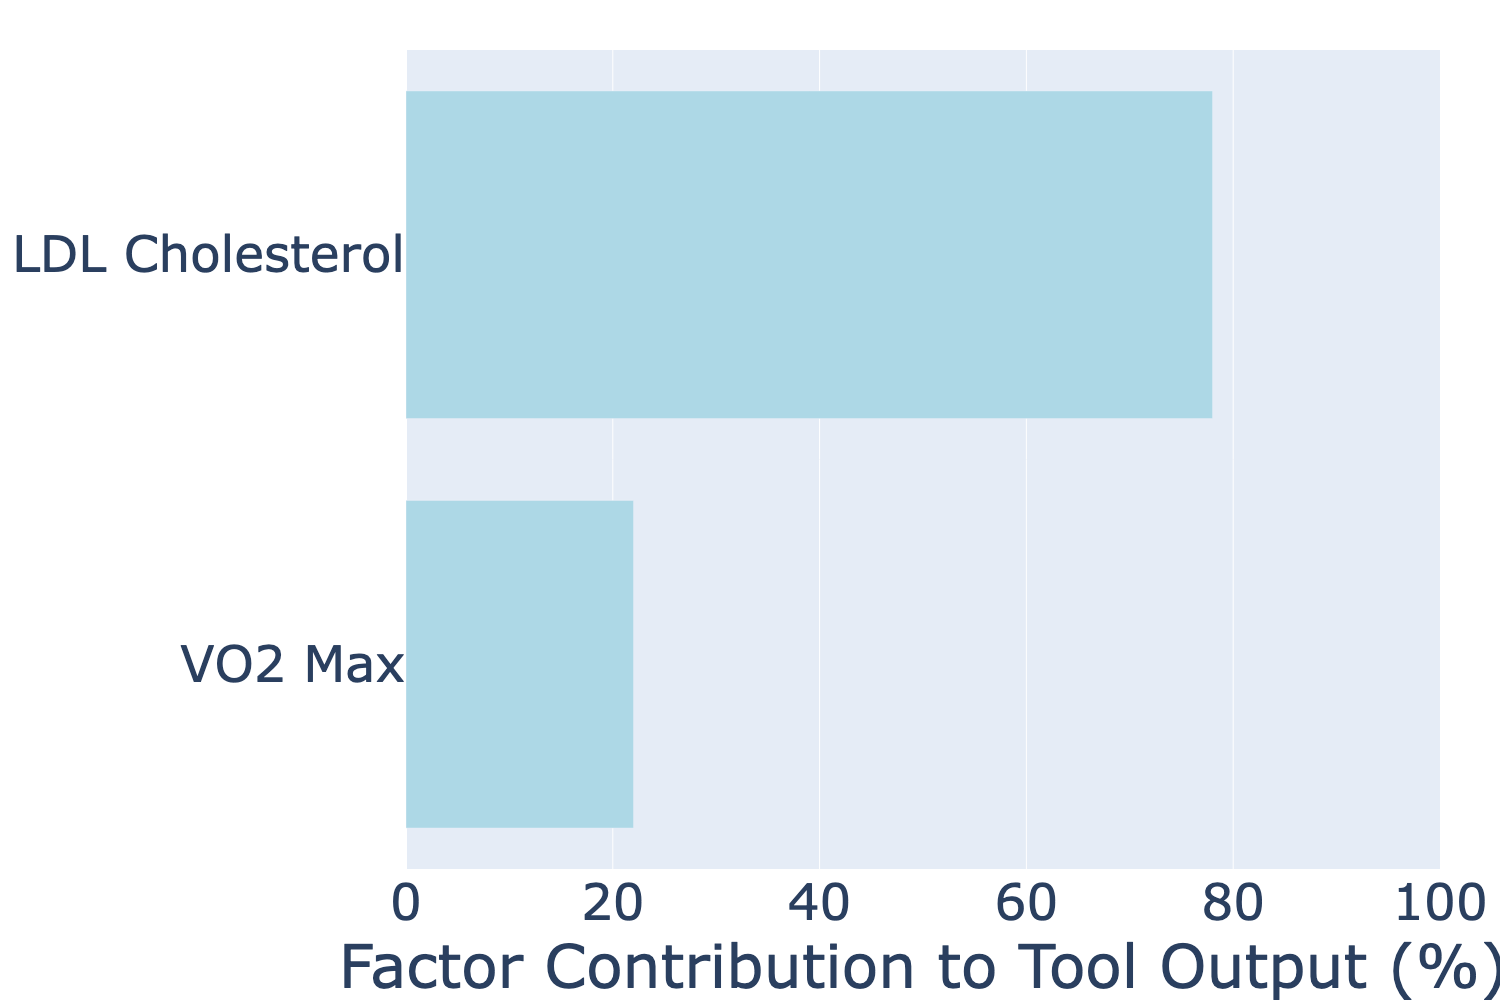
\includegraphics[width=0.24\textwidth]{Figures/2_unf_unbal.png}
    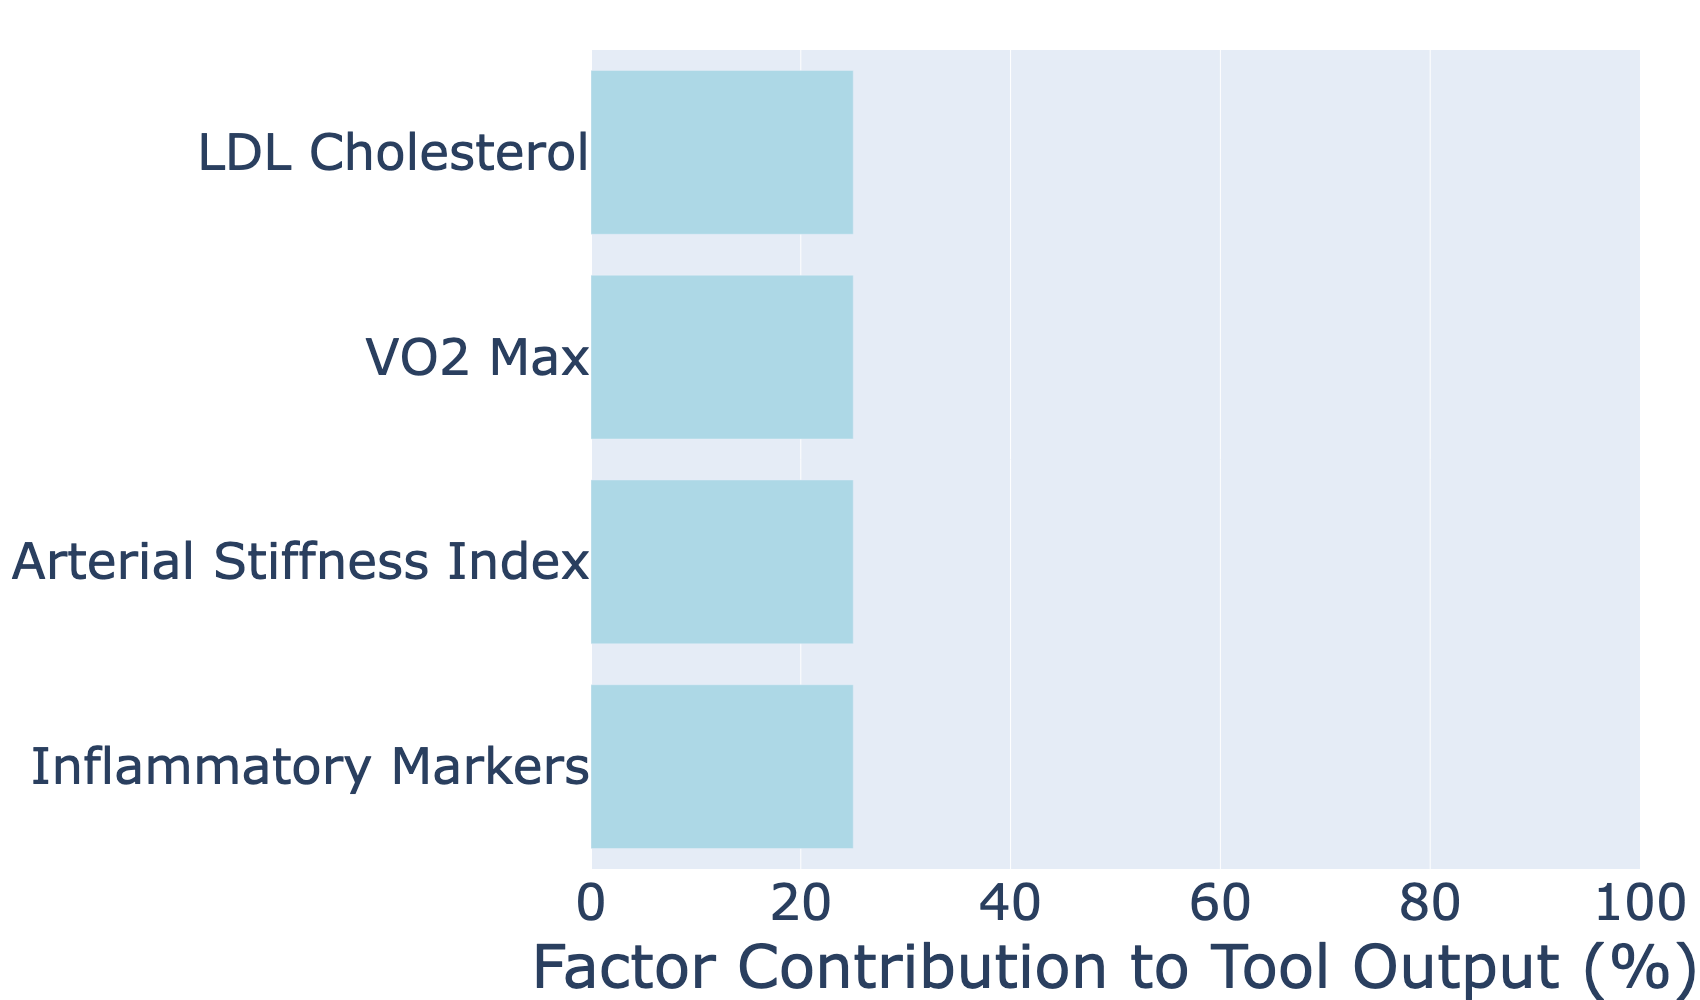
\includegraphics[width=0.24\textwidth]{Figures/4_unf_bal.png}
    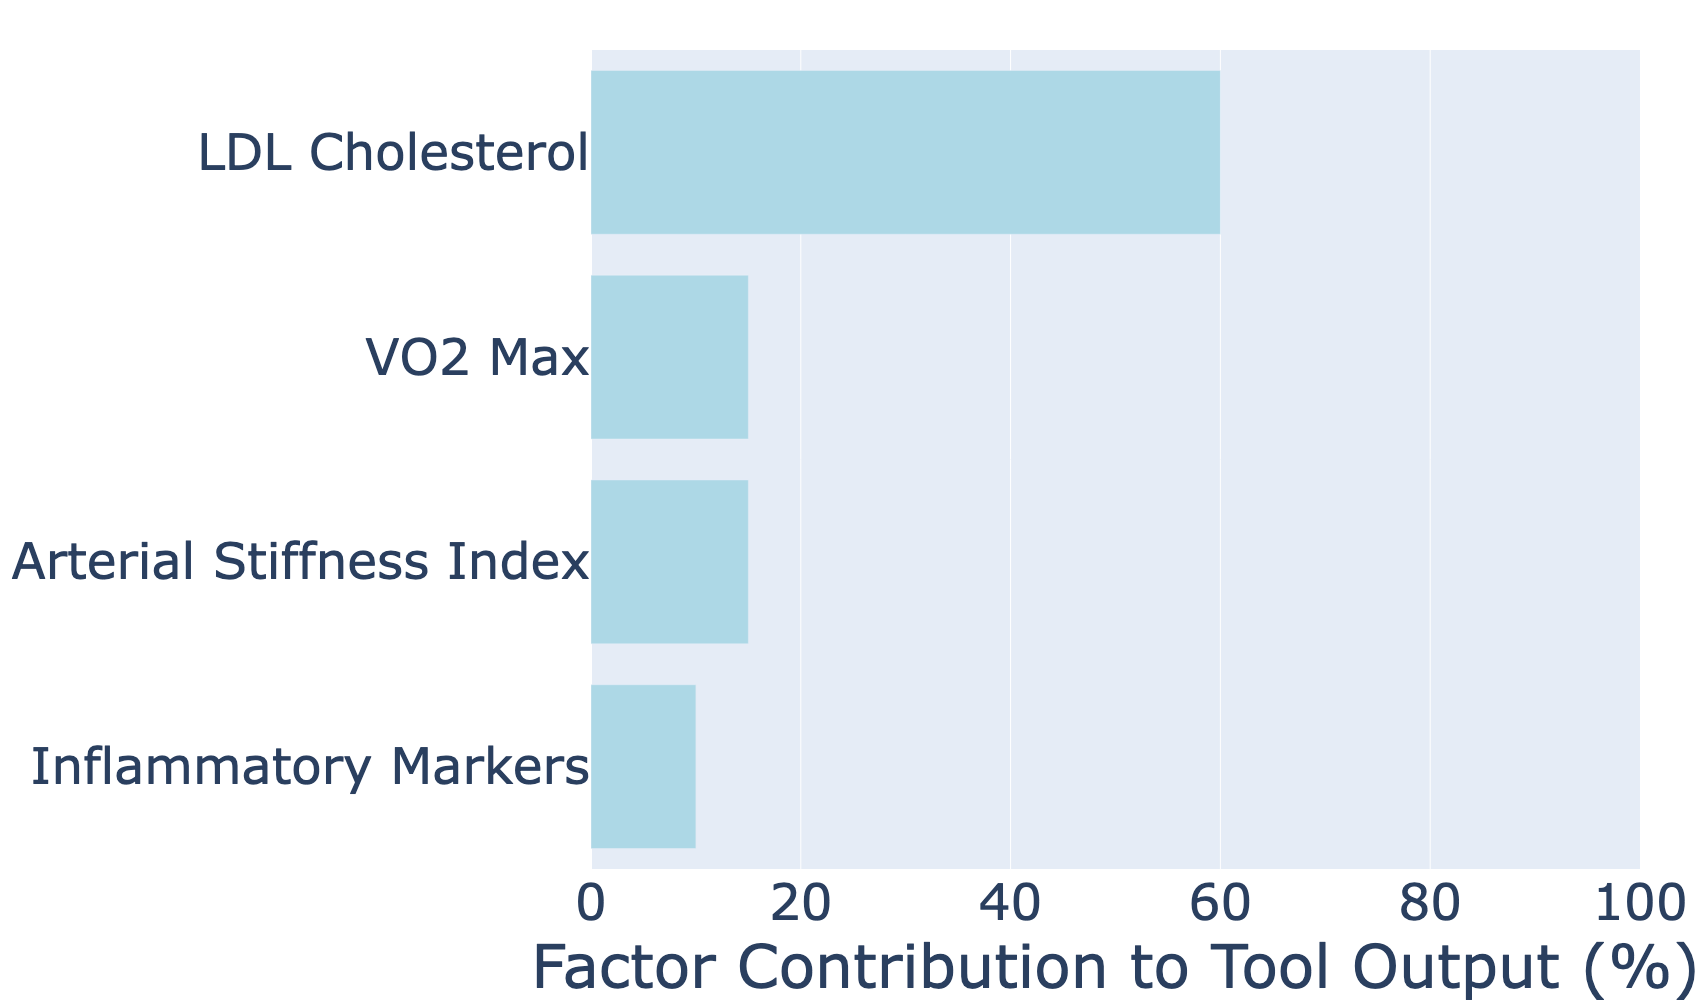
\includegraphics[width=0.24\textwidth]{Figures/4_unf_unbal.png}
    
    \caption{The scenarios shown to participants with familiar context in the first row and unfamiliar context in the second row: two or four features of similar importance (first and third column of figures from the left resp.), and two or four features of differing importance (second and last column of figures from the left resp.).}
    \Description[Survey plots]{The scenarios shown to participants: two or four features of similar importance (top and bottom left resp.), and two or four features of differing importance (top and bottom right).}
    \label{fig:feature-based-explanations}
\end{figure*}


\noindent\textbf{Task.} The familiar task asked participants to give advice to a friend about how to prepare for the job application process. Participants were told an AI system provides predictions of applicants' qualification for the job. The features used by the AI were resume (R) and cover letter (CL), with two additional features, interview (I) and LinkedIn profile (LP), for the four feature conditions. The unfamiliar task asked participants to give a friend advice about how to improve health metrics for a medical test. Participants were told an AI system provides predictions of the likelihood of a major cardiovascular event. The features used by the AI were LDL cholesterol (L) and VO2 max (V), with two additional features, arterial stiffness index (A) and inflammatory markers (I), for the four feature conditions.

Each participant had a budget (10 hours in the familiar context and 10 weeks in the unfamiliar context) to allocate between the given features to improve the likelihood of favorable recommendation. For starting features, in the two-feature and four-feature scenarios, we used $\vx_0=(40, 60)$ and $\vx_0=(60, 40, 60, 65)$, where, the maximum for feature scores is 100. For each hour allocated to any feature, participants were given a piecewise linear cost: the feature's score improves by 5 points for the first four hours, 2.5 points for the second four hours, and 1 point for extra hours after that. 

\noindent\textbf{Correct (``optimal'') answers.} For two balanced features, one should \emph{not} invest more than 6 hours in any feature. In the familiar (unfamiliar) context scenario with two unbalanced features, the optimal investments in the resume (LDL cholesterol) and cover letter (VO2 max) are 8 hours and 2 hours, respectively. For the familiar (unfamiliar) context scenario with four balanced features, the optimal is to invest at most 4 hours in any feature. For the familiar (unfamiliar) unbalanced four features case, the optimal investment is to allocate 8 hours to the interview LDL cholesterol) and the remaining 2 hours to the resume (VO2 max) and cover letter (arterial stiffness index). In this case, any investment in the LinkedIn profile (Inflammatory markers) feature is sub-optimal. A more detailed explanation is given in Appendix~\ref{sec:app-piece-wise-sol}. 

\noindent\textbf{Measures.} For other dependent measures, we used self-reported measurements of satisfaction, understanding, trust, and task performance using five-point semantic scales. We lightly edited questions from \cite{mohseni2021survey} for brevity and clarity.

\noindent\textbf{Recruitment.} We recruited 100 participants for familiar context through Prolific in September 2024 and 100 participants for unfamiliar context in January 2025. Quotas on education level and gender ensured the sample was representative of the United States. Additionally, we gathered demographic information and assessed participants' familiarity with machine learning to ensure a representative and unbiased sample.


\subsection{Results and Discussion}\label{sec:user-study-results}
\textbf{Adding complexity reduces performance.} Our findings indicate that participant performance decreases when we increase the number of features from two to four or shift from balanced to unbalanced feature weights. We evaluate performance by comparing the total score of a response to the optimal total score for that case. The total score of each response is calculated by first determining the new feature vector $\vx$ by adding the improvements of each feature to $\vx_0$ based on the subject's response, and then calculating $\vtheta^T\vx$. 

\begin{figure}[ht]
    \centering
    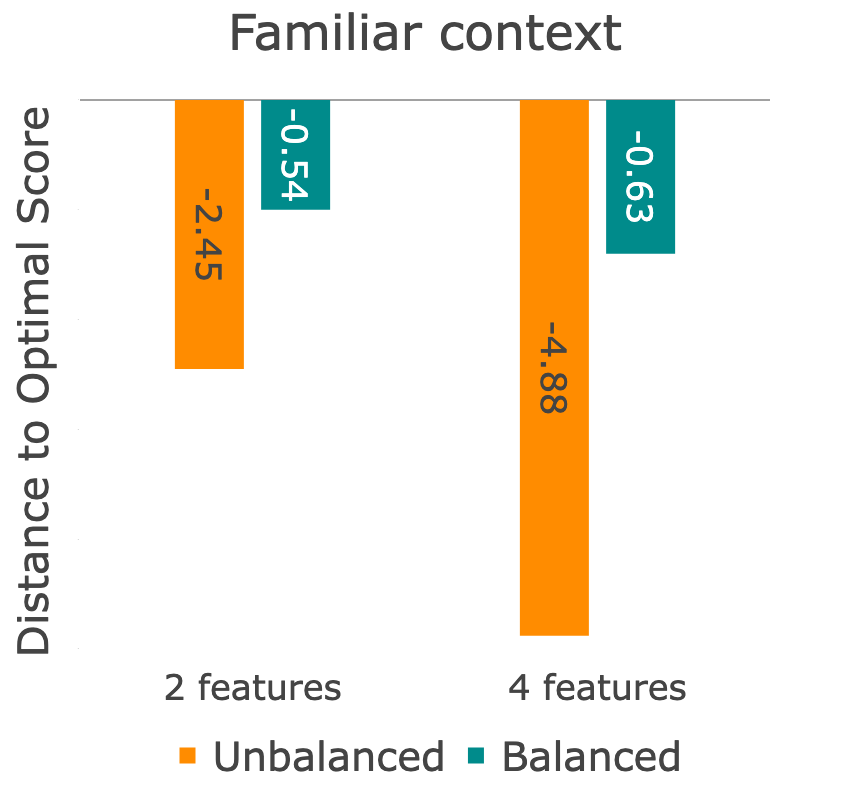
\includegraphics[width=0.2\textwidth]{Figures/distance_fam.png}
    \hspace{0.2in}
    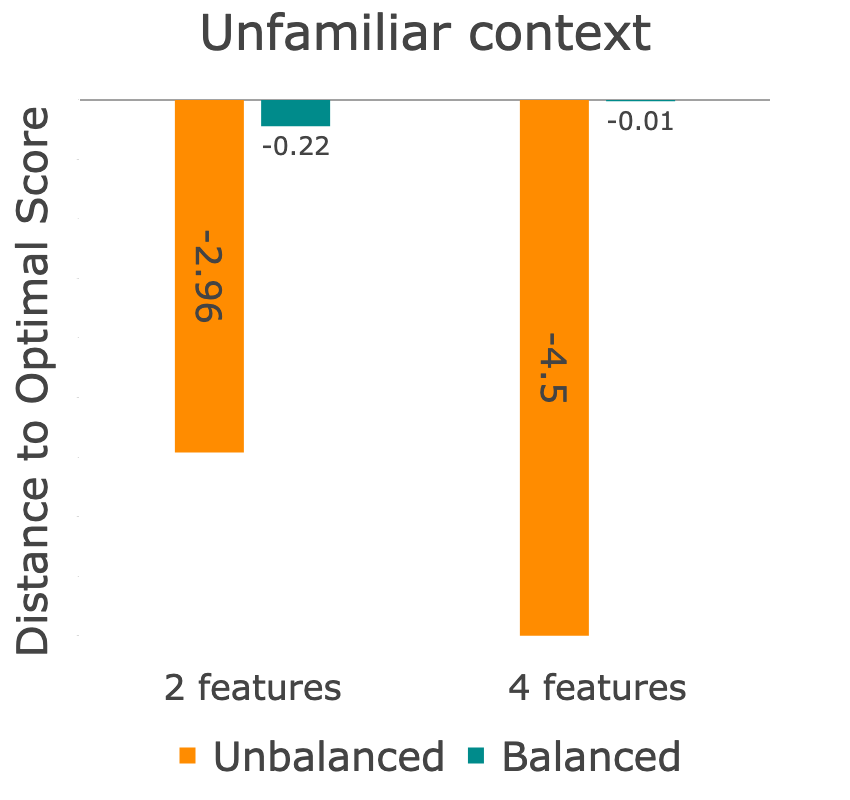
\includegraphics[width=0.2\textwidth]{Figures/distance_unf.png}
    \caption{The average distance to optimal ($\vtheta^T\vx_\text{NB}-\vtheta^T\vx_\text{B}$) for the four scenarios and two contexts.}
    \Description[Survey results showing the distance to optimal]{The average distance to optimal ($\vtheta^T\vx_\text{NB}-\vtheta^T\vx_\text{B}$) for the four scenarios.}
    \label{fig:dist-to-opt}
\end{figure}


In Figure~\ref{fig:dist-to-opt}, we observe that in the familiar context scenarios as the number of features increases, adding more complexity to the model, participants will move further away from the optimal score in balanced and unbalanced cases. The increase in the unbalanced case is almost double that of the balanced case. This indicates that we observe behavioral responses even in the balanced case, indicating biases beyond those in our theoretical predictions. For a fixed number of features, we see that answers are far from optimal when we have unbalanced features. Increasing the number of features will also lead to worse answers. On the other hand, in the unfamiliar context scenario we see the same pattern and numbers for unbalance features. However, with balanced features, the distance from optimal decreases compared to the familiar case. This could be a result of agents relying more on the model and the explanation when the context becomes unfamiliar and therefore respond more rationally. This does not necessarily mean that relying on the model in an unfamiliar context is better. Over reliance on AI models can also be problematic \cite{vasconcelos2023explanations, passi2022overreliance, buccinca2021trust}.

\begin{table}[ht]
    \caption{Number of responses in each scenario, (B) balanced and (U) unbalanced features for familiar context} 
    \label{table:number-of-responses-fam}
    \begin{center}
        \begin{tabular}{llll}
        \textbf{Scenario (familiar)}  &\textbf{Opt.} &\textbf{1-feature} &\textbf{Sub-opt.} \\
        \hline \\[-4.8pt]
        2-features (B) & 21 & 0 & 6 \\
        4-features (B) & 14 & 1 & 10 \\
        2-features (U) & 5 & 3 & 16 \\
        4-features (U) & 1 & 1 & 22
        \end{tabular}
    \end{center}
\end{table}

\begin{table}[ht]
    \caption{Number of responses in each scenario, (B) balanced and (U) unbalanced features for unfamiliar context} 
    \label{table:number-of-responses-unf}
    \begin{center}
        \begin{tabular}{llll}
        \textbf{Scenario (unfamiliar)}  &\textbf{Opt.} &\textbf{1-feature} &\textbf{Sub-opt.} \\
        \hline \\[-4.8pt]
        2-features (B) & 24 & 0 & 4 \\
        4-features (B) & 23 & 0 & 5 \\
        2-features (U) & 5 & 0 & 26 \\
        4-features (U) & 0 & 1 & 31
        \end{tabular}
    \end{center}
\end{table}

Table~\ref{table:number-of-responses-fam} shows that not only does the average distance from the optimal score increase with added complexity, but also the number of participants that responded sub-optimally increases. Most participants could find the optimal answers in the balanced cases, but most responded sub-optimally in the unbalanced cases. On the other hand, Table~\ref{table:number-of-responses-unf} indicates no significant difference in the number of people who responded sub-optimally to 2-feature and 4-feature conditions in the balanced case. However, we see The same pattern as in Table~\ref{table:number-of-responses-fam} for the unbalanced case.

\textbf{Participants exhibit different behavioral biases.} 
The unbalanced scenarios suggest that the behavior of most participants aligns with a Prelec function when (mis)perceiving feature importance. Specifically, the sub-optimal responses provided by the majority of participants would be considered optimal if the weights were adjusted according to Prelec function with $\gamma\le 0.64$ for two features scenario and $\gamma\le 0.55$ for four features scenario. This indicates that their decision-making may be systematically influenced by distorted perceptions of feature importance, consistent with the characteristics of the Prelec function. This leads them to under-invest in the most important feature and over-invest in the least important one. Participants not following the Prelec function tend to allocate all their budget to the most important feature.


The results from the balanced scenarios shed light on another behavioral bias: In the case of similar importance, participants invest more in the feature with a lower starting point (the resume in familiar context and VO2 max in the unfamiliar context). In the balanced scenarios, we notice that most participants respond without a behavioral bias, as predicted by the bias and Prelec functions. However, some participants responded sub-optimally, all over-investing in the feature with a lower starting point (resume or VO2 max). In the unbalanced four-feature case with familiar context, the average investment in the resume is higher despite the resume and the cover letter having the same importance, same statement is true for unfamiliar case and VO2 max and arterial stiffness index, indicating that this occurs for any two features with the same weight regardless of the importance of other features or the context. 

Focusing on the unbalanced scenarios, we see that the number of participants who respond with the optimal answer drops when we increase the number of features. More participants decide to invest all their budget in the most important feature. Findings from the unbalanced two-feature scenario show that if participants do not invest all their budget in the most important feature, they under-invest in it. 

\begin{table}[ht]
    \caption{Average distance of investment in most important and least important features in unbalanced scenarios from the optimal.}\label{table:avg-dist-from-opt}
    \begin{center}
        \begin{tabular}{lll}
         &\textbf{Most important} &\textbf{Least important} \\
        \hline \\[-4.8pt]
        2-features (Familiar) & -2.13 hours & +2.13 hours \\
        2-features (Unfamiliar) & -2.26 hours & +2.26 hours \\
        4-features (Familiar) & -4.11 hours & +1.76 hours \\
        4-features (Unfamiliar) & -3.90 hours & +1.64 hours
        \end{tabular}
    \end{center}
\end{table}
Assuming the Prelec function, we find that $\gamma$ for the participants answering the unbalanced two-features scenario is $\gamma \le 0.64$, vs. $\gamma\le 0.55$ for four-features. (The lower the $\gamma$ in the Prelec function, the more intense the bias.) These upper bounds come from the fact that participants must underestimate the importance of the most important feature enough so that they conclude it is better to invest in the second most important feature.  

Another interesting observation in the unbalanced four-features scenario is that, even though any investment in the least important feature was sub-optimal, 18 participants in the familiar context and 27 participants in the unfamiliar context still invested. This could be either a result of participants overestimating the importance of the least important feature, or a different behavioral bias, where participants prefer to invest in all options, and avoid leaving any feature as is. {A more detailed statistical report of the user study is included in Appendix~\ref{sec:app-stats-survey}}
